\begin{topic}{HTTP: Hypertext Transfer Protocol}

Application protocol for websites.

\textbf{Client requests} web objects from server.

\textbf{Server responds} with web objects when requested.

HTTP uses TCP connections (port 80)

HTTP is a \textbf{stateless protocol}. Server does not maintain client information.

\textbf{Persistent HTTP} allows \textbf{multiple objects} per connection. 


\end{topic}

\begin{topic}{Non-persistent HTTP}

\textbf{Non-persistent HTTP} restricts \textbf{one object} per connection.

\begin{enumerate}
	\item Client makes TCP connection to port 80 using a socket
	\item Server accepts incoming TCP connection
	\item Client sends request message over socket to access a resource
	\item Server responds with requested resource
	\item Server closes connection
	\item Client receives requested resource
\end{enumerate}

\end{topic}

\begin{topic}{Non-persistent HTTP Time}

\begin{multicols}{2}
\textbf{RTT:} time for a packet to travel from a client to a server and back.

\textbf{Non-persistent Response Time = } initial RTT + request RTT + file transmission time

\columnbreak
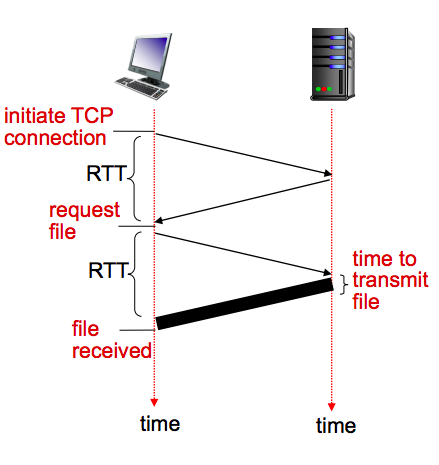
\includegraphics[scale=0.35]{coms3200/images/nonpersistent}
\end{multicols}

\end{topic}

\begin{topic}{Persistent HTTP}

Non-persistent HTTP requires 2 RTTs + OS overheard for each object.

\textbf{Persistent HTTP} leaves connections open allowing for as little as 1 RTT per object.

\end{topic}

\begin{topic}{HTTP Messages}

There are \textbf{request} and \textbf{response} HTTP messages

\begin{subtopic}{2}
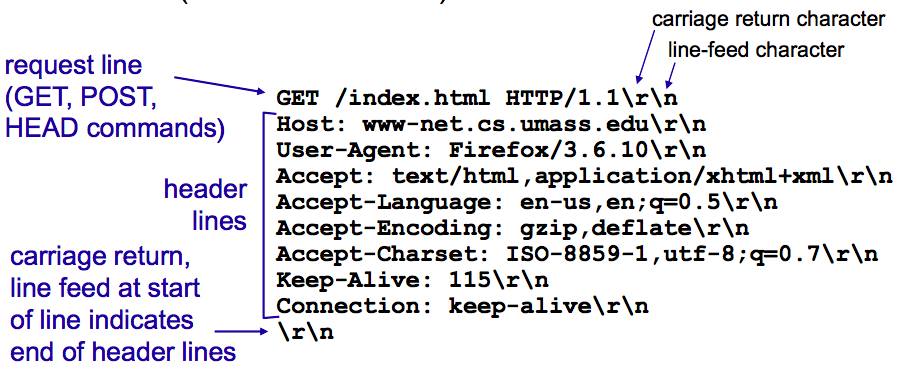
\includegraphics[scale=0.35]{coms3200/images/request}
\end{subtopic}

\begin{subtopic}{3}
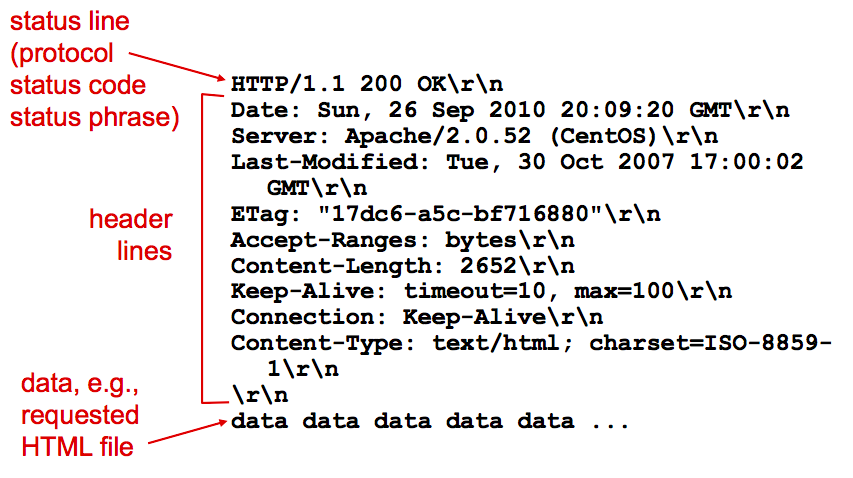
\includegraphics[scale=0.35]{coms3200/images/response}
\end{subtopic}

\begin{subtopic}{4}
\textbf{Method Types}
\begin{multicols}{2}
\textbf{HTTP 1.0 Methods:} GET, POST, HEAD

\textbf{HEAD} asks the server to not send back the requested object.

\columnbreak

\textbf{HTTP 1.1 Methods:} GET, POST, HEAD, PUT, DELETE

\textbf{PUT} uploads object to the given URL

\textbf{DELETE} deletes object at given URL
\end{multicols}
\end{subtopic}

\begin{subtopic}{5}
\textbf{Response Codes}

\begin{itemize}
	\item 200 OK
	\item 301 Moved Permanately
	\item 400 Bad Request
	\item 404 Not Found
	\item 505 HTTP Version Not Supported
\end{itemize}

\end{subtopic}

\end{topic}

\begin{topic}{Cookies and Caches and Conditional GETs}
... oh my!

Skipping for now
\end{topic}